\documentclass[12pt, dvipdfmx]{beamer}

\renewcommand{\kanjifamilydefault}{\gtdefault}
%%%%%%%%%%%  package  %%%%%%%%%%%
\usepackage{bxdpx-beamer}% dvipdfmxなので必要
\usepackage{pxjahyper}% 日本語で'しおり'したい

\usepackage{amssymb,amsmath,ascmac}

\usepackage{multirow}
\usepackage{bm}

\graphicspath{{../../../Figures/gakkai/}}

\usepackage{tikz}
\usepackage{xparse}

\usepackage{multimedia}

\usetikzlibrary{shapes,arrows}
%% define fancy arrow. \tikzfancyarrow[<option>]{<text>}. ex: \tikzfancyarrow[fill=red!5]{hoge}
\tikzset{arrowstyle/.style n args={2}{inner ysep=0.1ex, inner xsep=0.5em, minimum height=2em, draw=#2, fill=black!20, font=\sffamily\bfseries, single arrow, single arrow head extend=0.4em, #1,}}
\NewDocumentCommand{\tikzfancyarrow}{O{fill=black!20} O{none}  m}{
\tikz[baseline=-0.5ex]\node [arrowstyle={#1}{#2}] {#3 \mathstrut};}

%微分関連のマクロ
%
\newcommand{\diff}{\mathrm d}
\newcommand{\difd}[2]{\dfrac{\diff #1}{\diff #2}}
\newcommand{\difp}[2]{\dfrac{\partial #1}{\partial #2}}
\newcommand{\difdd}[2]{\dfrac{\diff^2 #1}{\diff #2^2}}
\newcommand{\difpp}[2]{\dfrac{\partial^2 #1}{\partial #2^2}}

%目次スライド
\AtBeginSection[]{
  \frame{\tableofcontents[currentsection]}
}

%アペンディックスのページ番号除去
\newcommand{\backupbegin}{
   \newcounter{framenumberappendix}
   \setcounter{framenumberappendix}{\value{framenumber}}
}
\newcommand{\backupend}{
   \addtocounter{framenumberappendix}{-\value{framenumber}}
   \addtocounter{framenumber}{\value{framenumberappendix}} 
}

\newcommand{\rmd}{\mathrm{d}}
\newcommand{\dd}[1]{\dfrac{\mathrm{d} #1}{\mathrm{d} x}}

%%%%%%%%%%%  theme  %%%%%%%%%%%
\usetheme{Copenhagen}
% \usetheme{Metropolis}
% \usetheme{CambridgeUS}
% \usetheme{Berlin}

%%%%%%%%%%%  inner theme  %%%%%%%%%%%
% \useinnertheme{default}

% %%%%%%%%%%%  outer theme  %%%%%%%%%%%
\useoutertheme{default}
% \useoutertheme{infolines}

%%%%%%%%%%%  color theme  %%%%%%%%%%%
%\usecolortheme{structure}

%%%%%%%%%%%  font theme  %%%%%%%%%%%
\usefonttheme{professionalfonts}
%\usefonttheme{default}

%%%%%%%%%%%  degree of transparency  %%%%%%%%%%%
%\setbeamercovered{transparent=30}

% \setbeamertemplate{items}[default]

%%%%%%%%%%%  numbering  %%%%%%%%%%%
% \setbeamertemplate{numbered}
\setbeamertemplate{navigation symbols}{}
\setbeamertemplate{footline}[frame number]

%%%%%%%%%%%%%%%%%%%%%%%%%%%%%%%%%%%
\title
% [ランダムな接続性を有するネットワークポリマーの緩和挙動]
{ランダムな接続性を有する\\ネットワークポリマーの緩和挙動}
\subtitle{補足資料}
\author[東亞合成 佐々木]{佐々木裕}
\institute[東亞合成]{東亞合成}
\date{October 21, 2021}
%%%%%%%%%%%%%%%%%%%%%%%%%%%%%%%%%%
\begin{document}
%%%%%%%%%%%%%%%%%%%%%%%%%%%%%%%%%%
\begin{frame}\frametitle{}
	\titlepage
\end{frame}

\section{これまでの検討結果}
\subsection{規則ネットワークでの検討}

% \subsection{これまでの検討結果}
\begin{frame}
	\frametitle{規則ネットワーク構造MDシミュレーション}
	\begin{columns}[totalwidth=1\textwidth]
		\column{.55\textwidth}
			ストランド長一定の規則構造
			\begin{itemize}
				\item 分岐数 
					\begin{itemize}
						\item 三分岐\\K4 構造
						\item 四分岐\\ダイヤモンド構造
					\end{itemize}
				\item ストランド
					\begin{itemize}
						\item KG鎖\\LJ ポテンシャルにより、排除体積効果を導入
						\item 素抜け鎖\\長距離相互作用を\\無視した理想鎖
					\end{itemize}
			\end{itemize}
		\column{.42\textwidth}
			\begin{itemize}
				\item K4 構造

				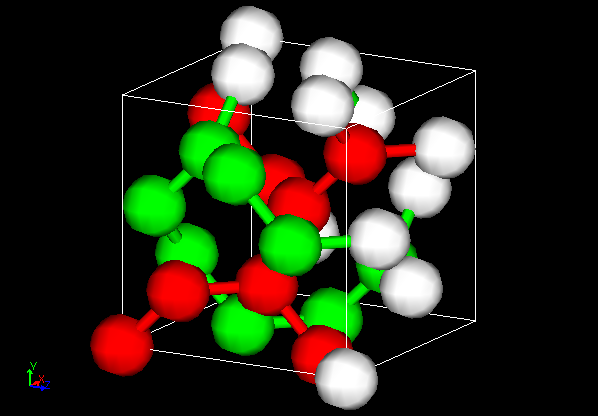
\includegraphics[width=0.8\textwidth]{K4_d.png}

				\item ダイヤモンド構造

				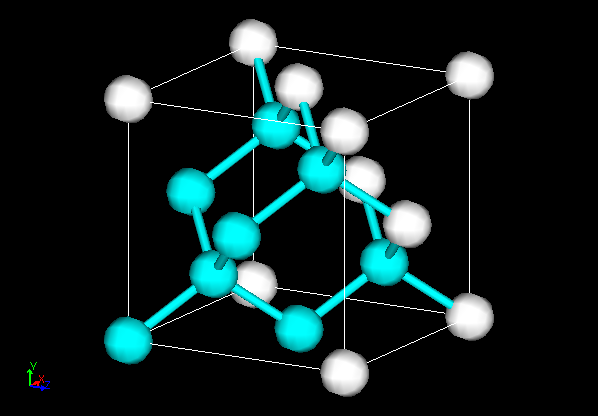
\includegraphics[width=0.8\textwidth]{dia.png}

			\end{itemize}
	\end{columns}
\end{frame}

\begin{frame}
	\frametitle{規則ネットワーク構造での検討結果}
		\small
		\begin{alertblock}{規則ネットワーク構造の振る舞い}
			\begin{itemize}
				\item 一軸伸長で、\alert{アフィンネットワークモデルの挙動}を示した
					\begin{itemize}
						\item \alert{分岐数、ストランドの性質(KG、素抜け)}によらず
				%	\item
				%	伸びきり効果をほぼ再現
					\end{itemize}
				\item 応力緩和で、主緩和が\alert{ラウスモードの最長緩和時間}程度
				\item 主緩和近傍に\alert{大きなエネルギー散逸($\tan \delta > 1$)}を確認
			\end{itemize}
		\end{alertblock}
		\begin{columns}[totalwidth=1\textwidth]
			\column{.32\textwidth}
				\scriptsize
				一軸伸長結果
				% \vspace{-2mm}
				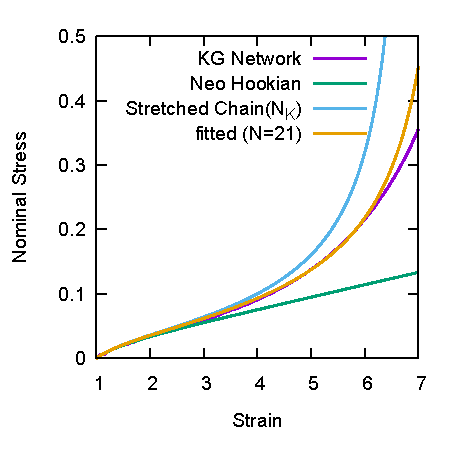
\includegraphics[width=0.9\textwidth]{SS_Kuhn.pdf}
			\column{.32\textwidth}
				\scriptsize
				応力緩和挙動
				% \vspace{-2mm}
				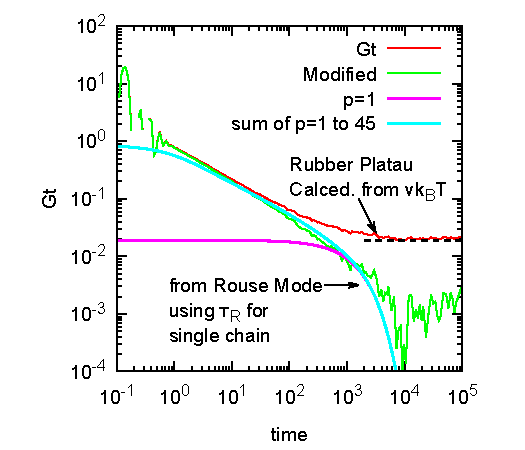
\includegraphics[width=0.9\textwidth]{Gt_loglog.pdf}
			\column{.32\textwidth}
				\scriptsize
				粘弾性スペクトル
				% \vspace{-2mm}
				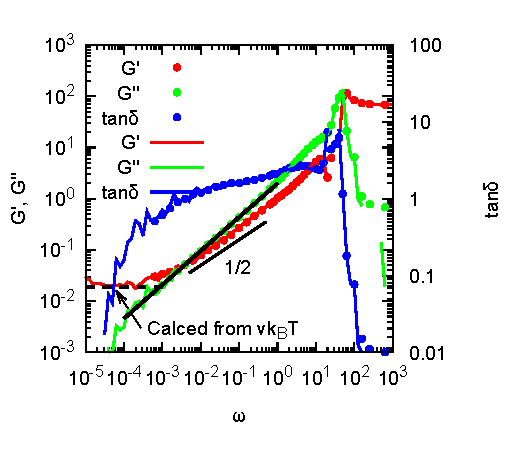
\includegraphics[width=\textwidth]{N_44_Freq_Sweep.pdf}
		\end{columns}
\end{frame}

\begin{frame}
	\frametitle{規則構造でのアフィン性}
		\begin{columns}[totalwidth=\linewidth]
			\column{.5\linewidth}
				\begin{block}{規則構造の特徴}
					\begin{itemize}
						\item 規則構造においては、\\結節点の\alert{連結性は等価}
							\begin{itemize}
								% \item それぞれの結節点の\\ゆらぎも等価
								\item 結節点は規則構造の\\平均位置に拘束
							\end{itemize}
						\item 巨視的な変形後
							\begin{itemize}
								\item 結節点の\alert{平均位置が\\アフィン移動}
								\item ゆらぎの異方性も類似
							\end{itemize}
					\end{itemize}
				\end{block}
			\column{.45\linewidth}
				規則構造の模式図
				\vspace{3mm}
				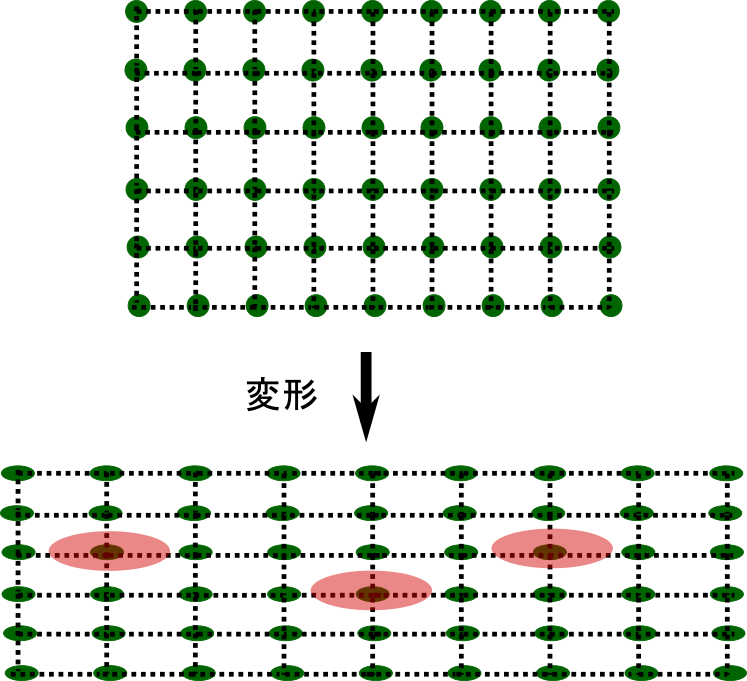
\includegraphics[width=\columnwidth]{reglar_NW_2.png}
		\end{columns}
		\begin{center}
			\Large
			\alert{緩和モードも単純}
		\end{center}
\end{frame}

\begin{frame}
	\frametitle{これまでの検討で出来ていないこと}
		\begin{alertblock}{規則構造でのシミュレーションでは}
			\begin{itemize}
				\item アフィンネットワークモデルでの単純な緩和挙動 
				\begin{itemize}
					\item ガラス転移終端近傍に主緩和
					\item ゆらぎの異方性が少ないためか?
				\end{itemize}
			\end{itemize}
		\end{alertblock}
		\begin{block}{ランダムネットワークの検討}
			\begin{itemize}
				\item ゆらぎの異方性を多様化したい
					\begin{itemize}
						\item ネットワーク構造の連結性にランダム性を導入
					\end{itemize}
				\item ランダムネットワークモデルの特徴
				\begin{itemize}
					\item アフィン変形を抑制?
				\end{itemize}
			\end{itemize}
		\end{block}
\end{frame}

\subsection{「す抜け鎖」のシミュレーション結果}
\begin{frame}
	\frametitle{「す抜け鎖」の力学応答}
		\begin{alertblock}{「す抜け鎖」でのランダムネットワーク}
			\begin{itemize}
				% \item ストランド:す抜け鎖
				\item 四分岐ランダムネットワークモデル
			\end{itemize}
		\end{alertblock}
		\begin{columns}[totalwidth=\linewidth]
			\column{.48\linewidth}
				\begin{block}{一軸伸張結果}
					\begin{itemize}
						\item 伸張速度低下でファントム応答に漸近
						% \item 低伸張率から伸び切り
					\end{itemize}
					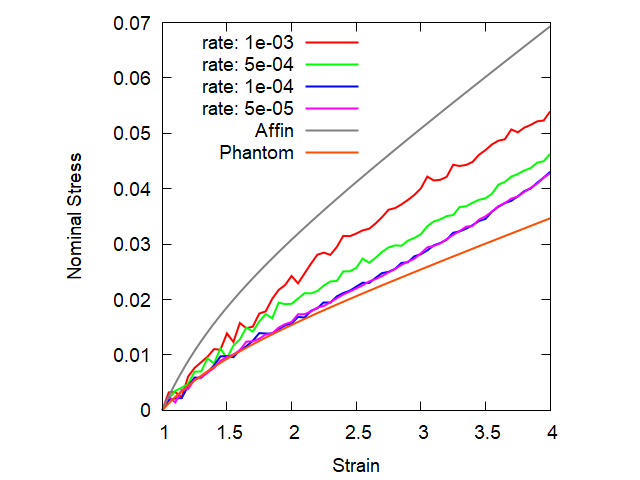
\includegraphics[width=.8\columnwidth]{N48_sunuke.png}
				\end{block}
			\column{.48\linewidth}
				\begin{exampleblock}{ステップ変形の応力緩和}
					% \begin{itemize}
					% 	\item 高速変形条件
							\begin{itemize}
								\item 高速伸長:$\dot{\gamma} = 1e^{-3}$
								\item 変位:$\lambda = 1.5$
							\end{itemize}
					% \end{itemize}
					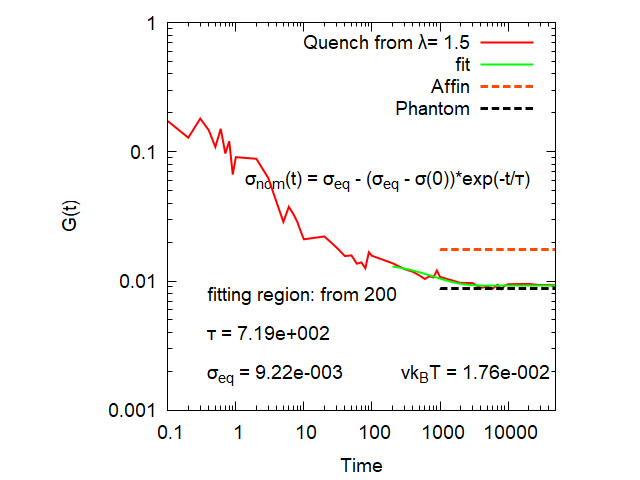
\includegraphics[width=.8\columnwidth]{gt_sunuke.png}
				\end{exampleblock}
		\end{columns}
\end{frame}

\subsection{ファントムネットワークの理論}
\begin{frame}
	\frametitle{有限サイズ効果}
		\begin{columns}[totalwidth=1\textwidth]
			\column{.48\textwidth}
				\begin{block}{末端の壁面固定の効果}
				\begin{itemize}
					\item 壁面に末端が固定
						\begin{itemize}
							\item $n$ 本のストランド
							\item セグメント数: $N$
							\item 他端が架橋点($\bm{r}$)
						\end{itemize}
					\item 架橋点の運動性
						\begin{itemize}
							\item 壁と$N/n$ 個の短い\\ストランドと等価
							\item 壁の移動(変形)の影響減少
						\end{itemize}
				\end{itemize}
				% \vspace{-2mm}
				\begin{center}
					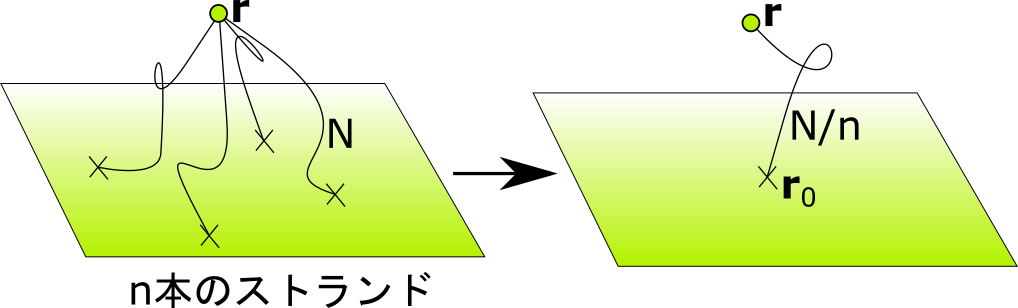
\includegraphics[width=.8\textwidth]{phantom-1.png}
				\end{center}
				\end{block}
			\column{.48\textwidth}
				\begin{exampleblock}{内部の鎖が受ける変形}
					\begin{itemize}
						\item システム内部の鎖の末端はガウス分布
						\item 壁面固定の末端からの変形が内部に伝達して、
					\end{itemize}
					\vspace{-3mm}
					\tiny
					\begin{align*}
						&G=\xi \nu k_BT \\
							&\begin{cases}
							\xi_{\infty} = 1-\dfrac{2}{f} \;\; \text{System}\sim \infty \\[8pt]
							\xi_{s} = \dfrac{f-1}{f+1} \;\; \text{Small Limit}
							\end{cases}
					\end{align*}
					\vspace{-5mm}
					\begin{center}
						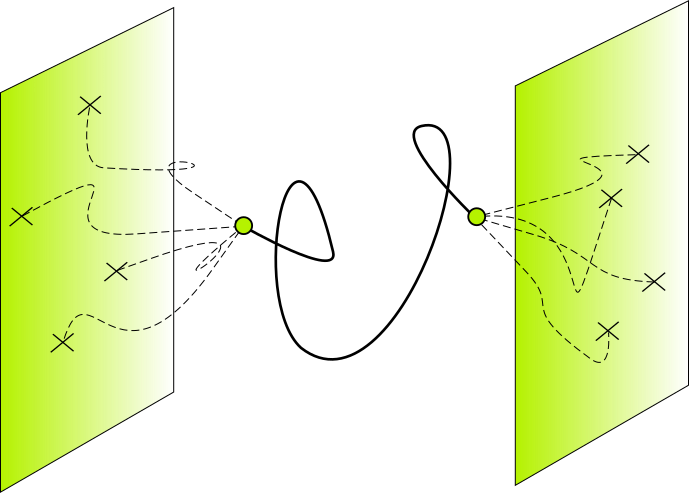
\includegraphics[width=0.5\textwidth]{phantom.png}
					\end{center}
				\end{exampleblock}
		\end{columns}
\end{frame}
% %%%%%%%%%%%%%%%%%%%%%%%%%%

% %%%%%%%%%%%%%%%%%%%%%%%%%%%%%%%%%%%%%%%%%%%%%%
% \subsection{ファントムネットワークの振る舞い}
\begin{frame}
	\frametitle{ファントムネットワークのゆらぎ}
		\begin{block}{ゆらぎの入ったポテンシャル}
			\begin{itemize}
				\item ストランドの末端間ベクトル $\bm{R}_{nm}$ を、\\架橋点の位置ベクトル $\bm{r}_n$ を用いて、
					\footnotesize
					\begin{equation*}
						\bm{R}_{nm} \equiv \bm{r}_n-\bm{r}_m
					\end{equation*}
					\normalsize
				\item 系のポテンシャルエネルギーは、
					\footnotesize
					\begin{equation*}
						U=\dfrac{k}{2} \sum_{\langle nm \rangle} \bm{R}_{nm}^2
					\end{equation*}
					\normalsize
				\item これは、自然長で決まる定数項と、ゆらぎに起因した第二項に分割でき、その和で以下となる。
					\footnotesize
					\begin{equation*}
						U=\dfrac{k}{2} \sum_{\langle nm \rangle} {\bm{R}_{nm}^{(0)}}^2 + \dfrac{k}{2} \sum_{\langle nm \rangle} \Delta \bm{R}_{nm}^2
					\end{equation*}
					\normalsize
			\end{itemize}
		\end{block}
\end{frame}

\begin{frame}
	\frametitle{ファントムネットワークのゆらぎ}
		\begin{block}{アンサンブル平均の二つの表式}
			\vspace{-5mm}
			\scriptsize
			\begin{align*}
				\begin{cases}
					\langle U \rangle = N_{strands} \dfrac{k}{2} \langle \Delta \bm{R}^2 \rangle \\
					\langle U \rangle = 3(N_{nodes}-1) \dfrac{1}{2} k_B T
				\end{cases}
			\end{align*}
			\normalsize
			なお、第二式は等分配側より導出した。
		\end{block}
		\begin{exampleblock}{ファントムネットワークでのゆらぎ}
			\begin{itemize}
				\item 架橋点数 $N_{nodes}$、架橋点官能基数 $f$ とすれば、
					\scriptsize
					\begin{equation*}
					\langle \Delta \bm{R}^2 \rangle = \dfrac{3k_B T}{k} \dfrac{2}{f} \left( 1-\dfrac{1}{N_{nodes}} \right)
					\end{equation*}
					\normalsize
				\item 適切な条件で、ストランドの自然長 $R_0$ を用いて、
					\scriptsize
					\begin{equation*}
					\color{red}
					\langle \Delta \bm{R}^2 \rangle = \dfrac{2}{f} R_0^2
					\end{equation*}
					\normalsize
			\end{itemize}
		\end{exampleblock}
\end{frame}



\section{ランダムネットワークの作成}

\subsection{ランダムネットワークの作成}
\begin{frame}
	\frametitle{トポロジーモデルへの変換}
		\begin{columns}[totalwidth=\textwidth]
			\column{.48\textwidth}
				\begin{block}{実空間での初期構造}
					\begin{itemize}
						\item $2\times2\times2$ 個の\\ユニットセル
			
							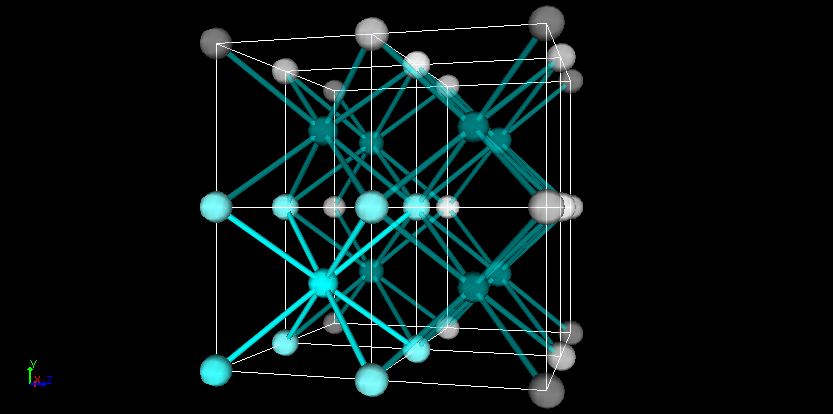
\includegraphics[width=0.8\columnwidth]{8_per.png}

						\item ユニットセルから除去

							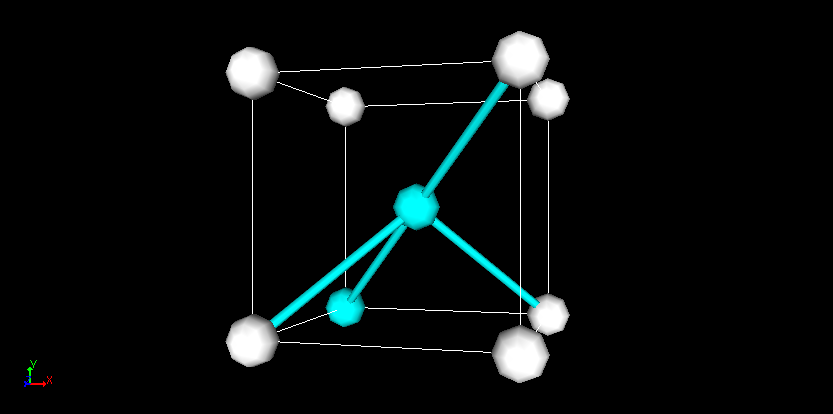
\includegraphics[width=0.8\columnwidth]{8_4.png}

					\end{itemize}
				\end{block}
		\column{.48\textwidth}
			\begin{exampleblock}{トポロジーモデル}
				分岐数を4に減じた\\トポロジーモデル

				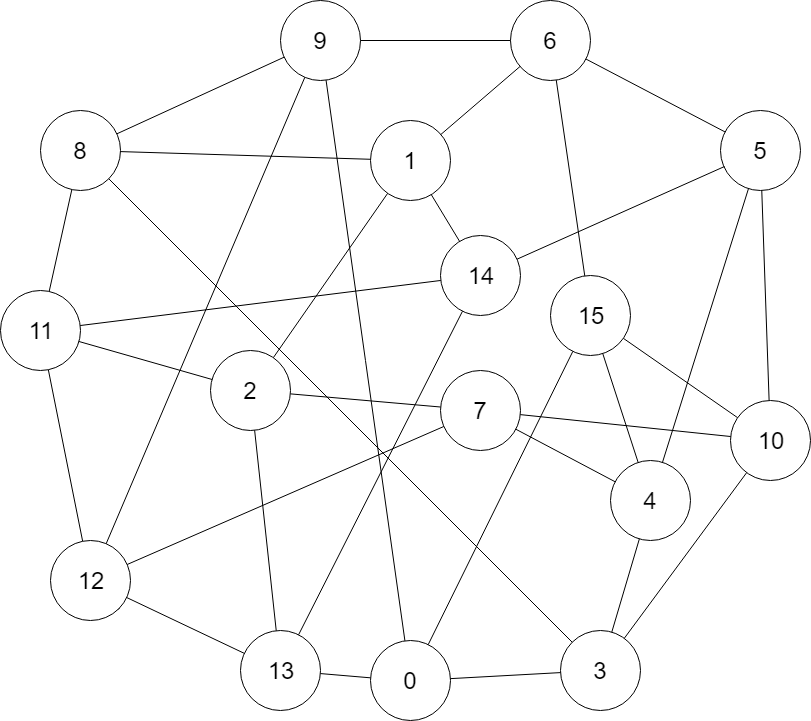
\includegraphics[width=\columnwidth]{Network.png}

			\end{exampleblock}
		\end{columns}
\end{frame}

\begin{frame}
	\frametitle{それぞれの分岐数での初期構造}
		\begin{exampleblock}{初期構造の作成}
			\begin{itemize}
				\item \alert{実空間}で8-Chain Model で初期構造を作成。
				\item 所望の分岐数に\alert{ランダム}に選択した\alert{結合を除去}
				\item 除去したジオメトリーに対応した\alert{トポロジーモデル}
			\end{itemize}
		\end{exampleblock}
		\begin{columns}[totalwidth=\linewidth]
			\column{.48\linewidth}
				\begin{block}{分岐数: 3, 4, 5 分岐}
					\begin{itemize}
						\item 3 分岐では、全てが連結していない
						\item 4 分岐では、連結していないものもある
						\item 5 分岐でも二種類のみ
					\end{itemize}
				\end{block}
			\column{.48\linewidth}
				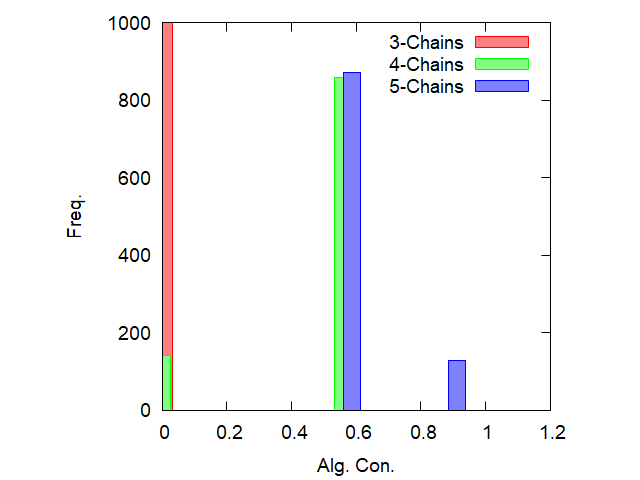
\includegraphics[width=\columnwidth]{Histgram2.png}
		\end{columns}
\end{frame}

\begin{frame}
	\frametitle{トポロジーモデルからのランダム性の導入}
		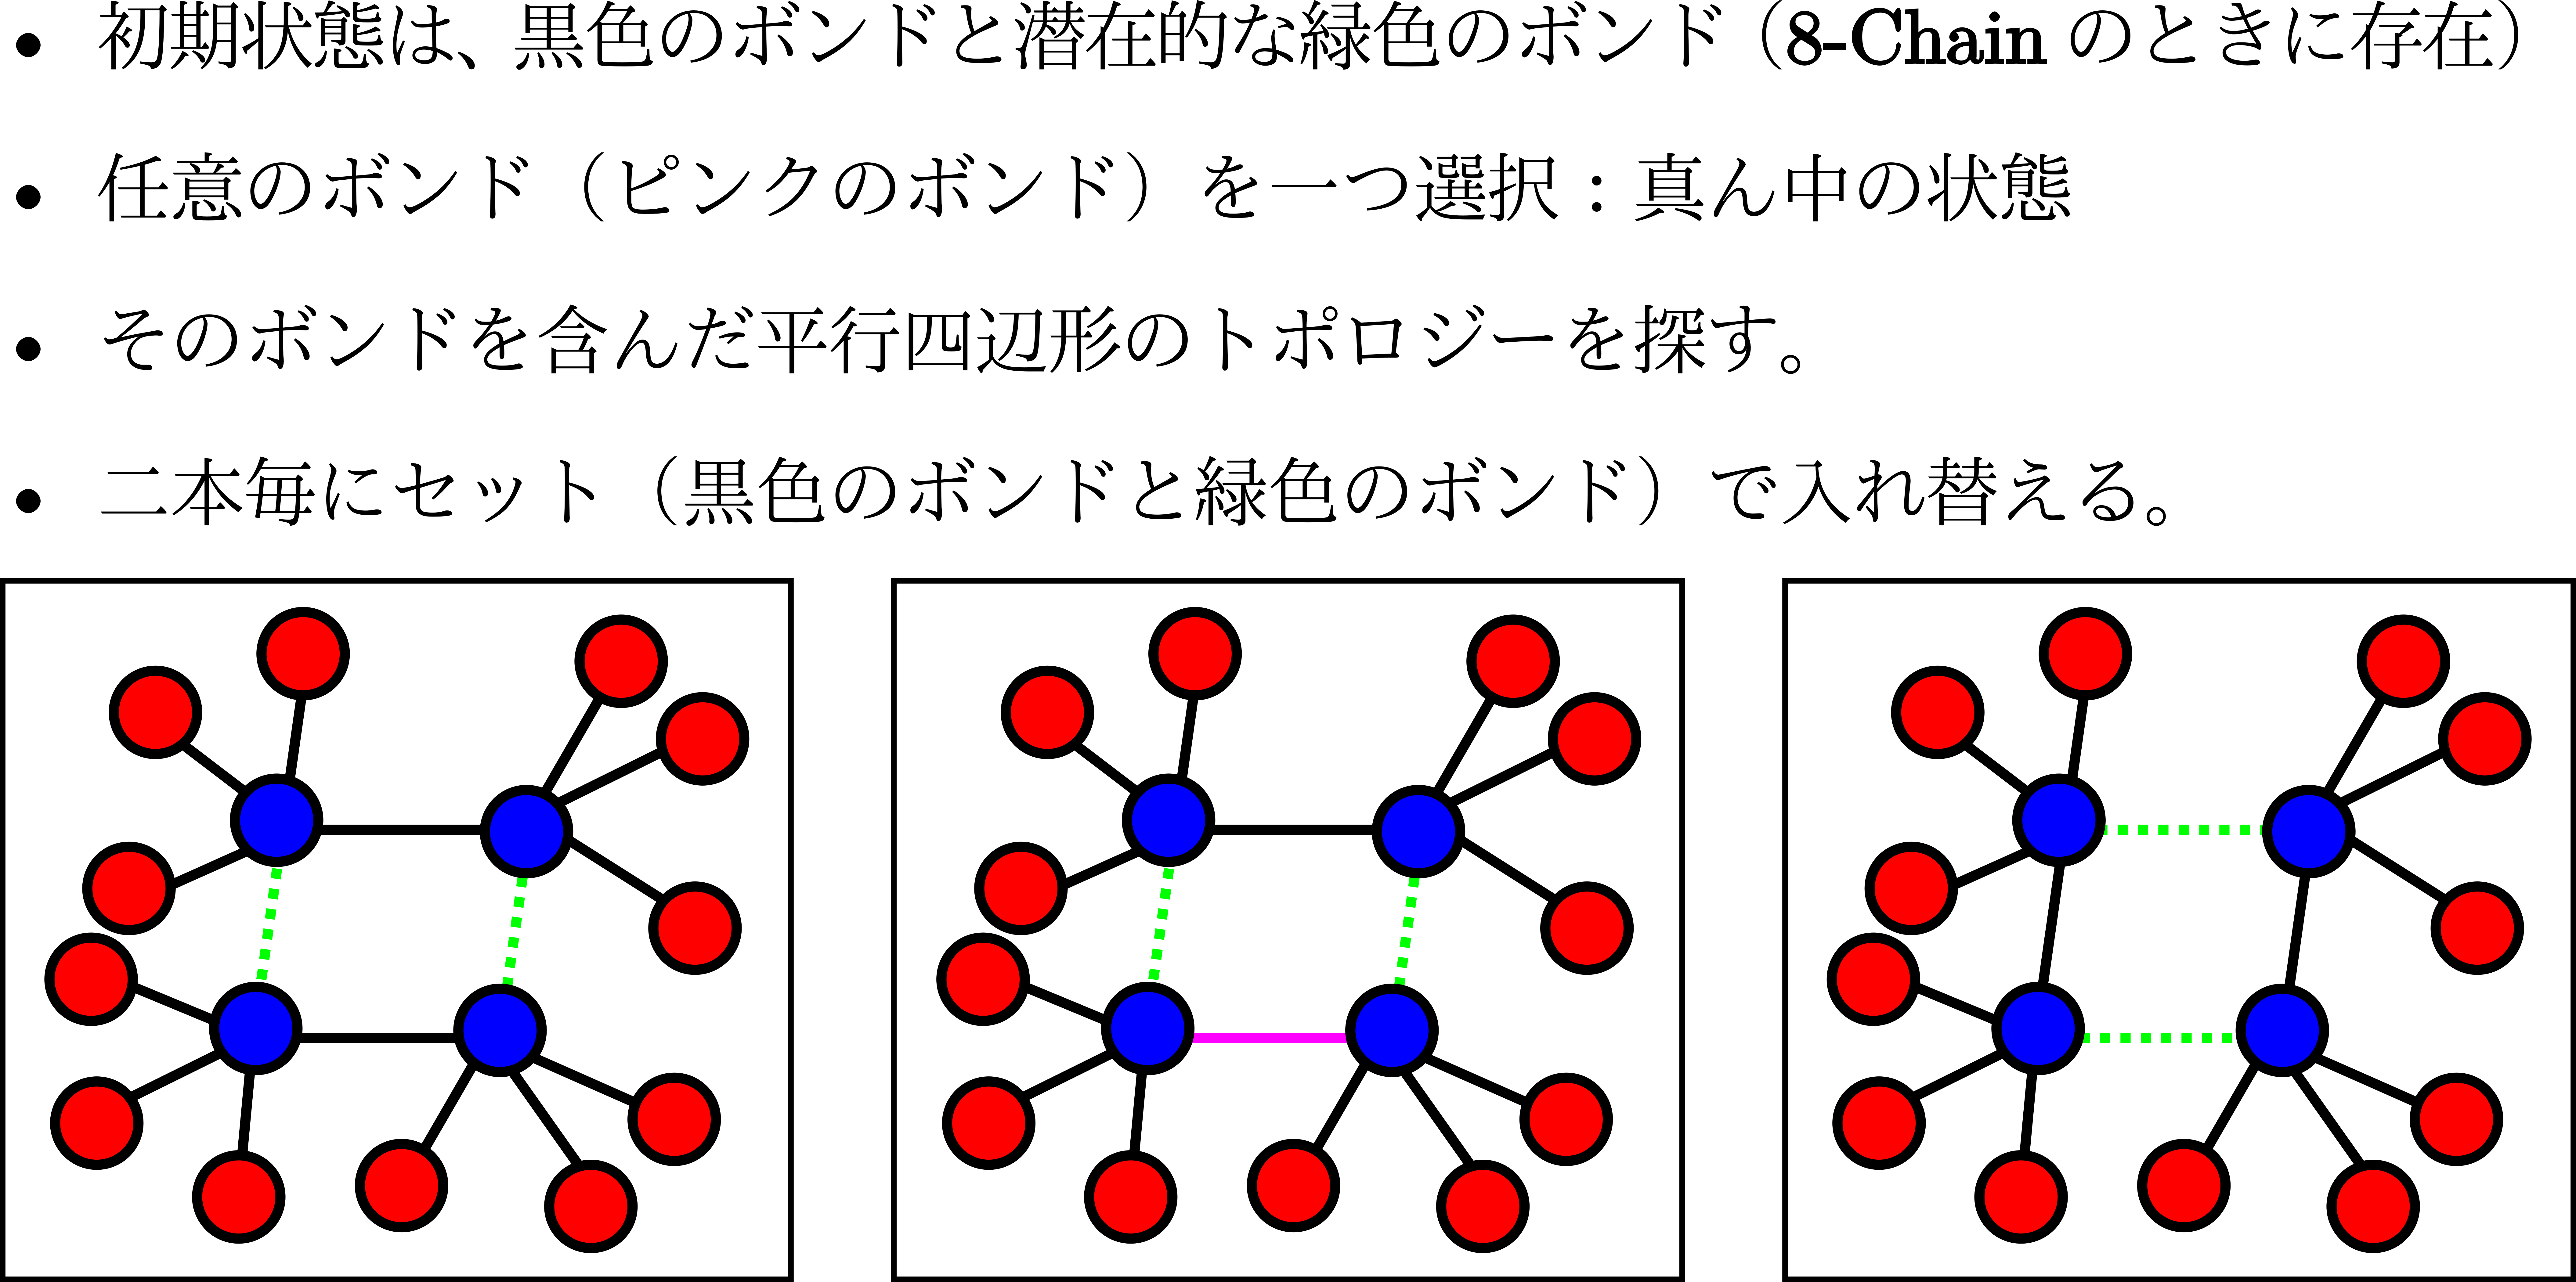
\includegraphics[width=\textwidth]{bond_exchg.png}
\end{frame}

\begin{frame}
	\frametitle{代数的連結性の分布関数}
		\begin{exampleblock}{サンプリング数の増加($> 1000,000$ times)}
			\begin{itemize}
				\item 3, 5分岐トポロジーモデルは、単鋒性に
				\item 4分岐のトポロジーモデルでは、二峰性\\
				サンプリング数を増やすと若干変化
			\end{itemize}
		\end{exampleblock}
		\begin{columns}[totalwidth=1\textwidth]
			\column{.33\textwidth}
				\begin{center}
					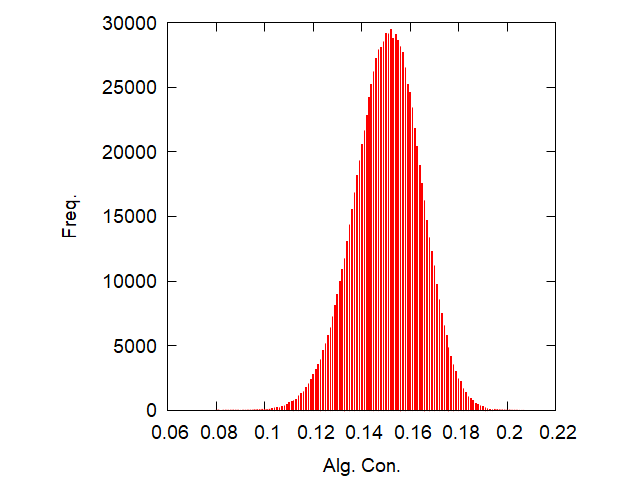
\includegraphics[width=1.2\columnwidth]{3.png}

					3-Chain Model
				\end{center}
			\column{.33\textwidth}
				\begin{center}
					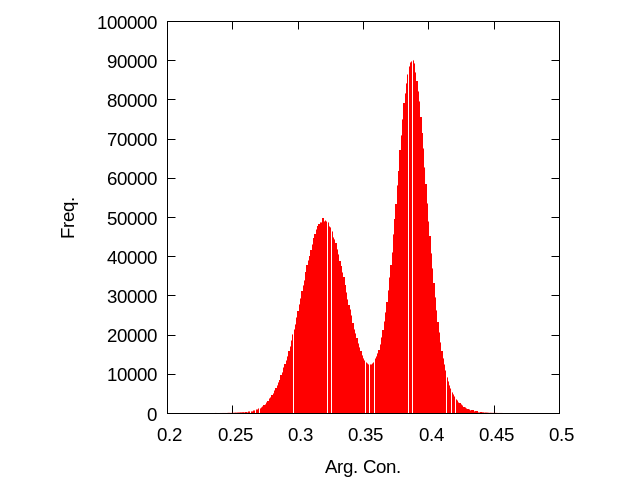
\includegraphics[width=1.2\columnwidth]{4_1000_5000.png}

					4-Chain Model
				\end{center}
			\column{.33\textwidth}
				\begin{center}
					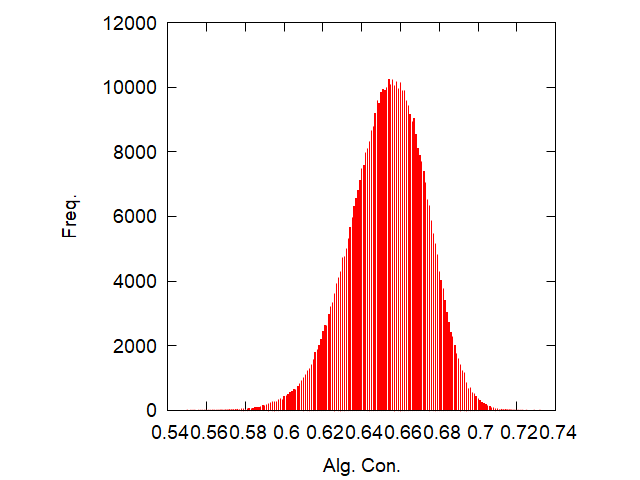
\includegraphics[width=1.2\columnwidth]{5.png}

					5-Chain Model
				\end{center}
		\end{columns}
\end{frame}


\subsection{ネットワークのトポロジー}
\begin{frame}
	\frametitle{ネットワークの分岐数の処理}
		以下のようにノード番号を付与したネットワークを考えると、
			\begin{center}
				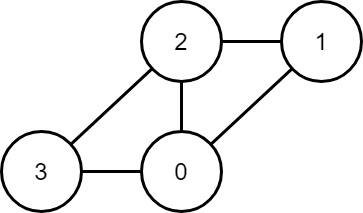
\includegraphics[width=4cm]{NW-4.png}
			\end{center}
		隣接行列、および、次数行列は、
		\begin{align*}
			A = \left( 
			\begin{array}{cccc} 
			0 & 1 & 1 & 1 \\ 
			1 & 0 & 1 & 0 \\
			1 & 1 & 0 & 1 \\
			1 & 0 & 1 & 0 
			\end{array} 
			\right) 
			,
			D = \left( 
			\begin{array}{cccc} 
			3 & 0 & 0 & 0 \\ 
			0 & 2 & 0 & 0 \\
			0 & 0 & 3 & 0 \\
			0 & 0 & 0 & 2 
			\end{array} 
			\right) 
		\end{align*}
		となる。
\end{frame}

\begin{frame}
	\frametitle{ラプラシアン行列}
		\begin{columns}[totalwidth=1\textwidth]
			\column{.48\textwidth}
				ラプラシアン行列は、隣接行列$A$と次数行列$D$により以下のように定義される。
				$$
				L \equiv D-A
				$$
				4つのノードからなるネットワークの例であれば、
				$$
				L = \left( 
				\begin{array}{cccc} 
				3 & -1 & -1 & -1 \\ 
				-1 &  2 & -1 & 0 \\
				-1 & -1 &  3 & -1 \\
				-1 &  0 & -1 & 2 
				\end{array} 
				\right) 
				$$
				となり、非負の固有値。
			\column{.48\textwidth}
				グラフが非連結であるとき、%ラプラシアン行列の成分を
				連結した成分ごとにブロック対角化できるので、固有値 0 の重複数がグラフの連結成分ブロックの総数となる。
				\begin{block}{「代数的連結性」}
					「グラフが連結である場合、ラプラシアン行列の固有値 0 の重複数は 1」となる。\\
					固有値を昇順にみた時、0 に次ぐ二番目の固有値がグラフの連結性の強さを示す指標となり、「代数的連結性」と呼ばれる。
				\end{block}
		\end{columns}
\end{frame}

\subsection{初期構造の緩和}
\begin{frame}
    \frametitle{初期構造の緩和}
        \vspace{-2mm}
		\begin{block}{KG 鎖をストランドとするネットワーク}
			\begin{itemize}
				\item KG鎖は「非素抜け」なので、\alert{初期構造の緩和}が重要。
				\vspace{-3mm}
					\fontsize{6pt}{0pt}
					\begin{align*}
						&U_{KG}(r) = 
						\begin{cases}
						U_{nonbond} = U_{LJ} \;\text{where } r_c = 2^{(1/6)}\sigma \\
						U_{bond} = U_{LJ} + U_{FENE}
						\end{cases} 
					\end{align*}
			\end{itemize}
		\end{block}
		\vspace{-3mm}
		\begin{columns}[totalwidth=\linewidth]
			\column{.7\linewidth}
				\begin{exampleblock}{初期構造の緩和}
					\begin{itemize}
						\item Auhl 等の方法に従い、
						\begin{itemize}
							\item force-capped-LJ ポテンシャル
							\item Slow Push Off で初期構造を緩和
						\end{itemize}
					\end{itemize}
					\vspace{-3mm}
					\fontsize{6pt}{0pt}
					\begin{align*}
						&U_{FCLJ}(r) = 
						\begin{cases}
						(r-r_{fc})*U_{LJ}^{\prime}(r_{fc}) + U_{LJ}(r_{fc}) \; &r< r_{fc} \\
						U_{LJ}   \;\;\;\;\;\;\; &r \geq r_{fc}
						\end{cases} 
					\end{align*}

                    \scriptsize{R. Auhl et al. J. of Chem. Phys., 119, 12718 (2003)}
				\end{exampleblock}
			\column{.28\linewidth}
				\vspace{2mm}
				\begin{center}
					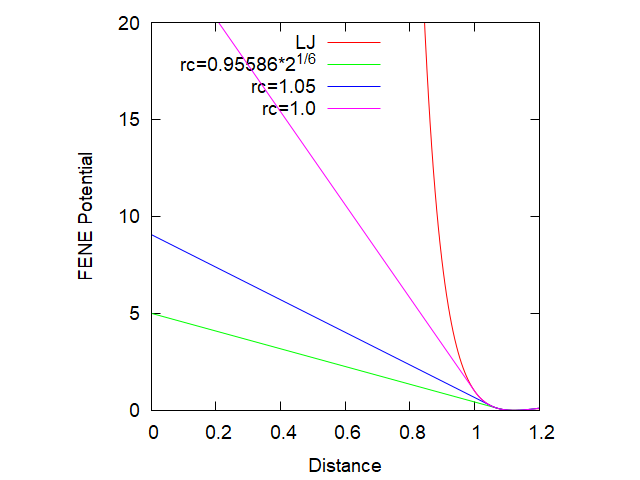
\includegraphics[width=\textwidth]{Ev_fcLJ.png}
				\end{center}
				\vspace{-3mm}
				\scriptsize
				\begin{itemize}
					\item force-capped-LJ Pot.
					\item 素抜け⇒絡み合い
				\end{itemize}
		\end{columns}
\end{frame}


\section{その他}
\subsection{絡み合いの評価}

\begin{frame}
	\frametitle{ランダムネットワークの絡み合い解析}
		\vspace{-6mm}
		\begin{columns}[T, onlytextwidth]
			\column{.48\linewidth}
			\begin{block}{N48 のネットワークのPPA}
				\begin{itemize}
					\item ストランド内部の非結合ポテンシャルを無効
					\item \alert{多数の絡み合いが存在}
				\end{itemize}
				\begin{center}
					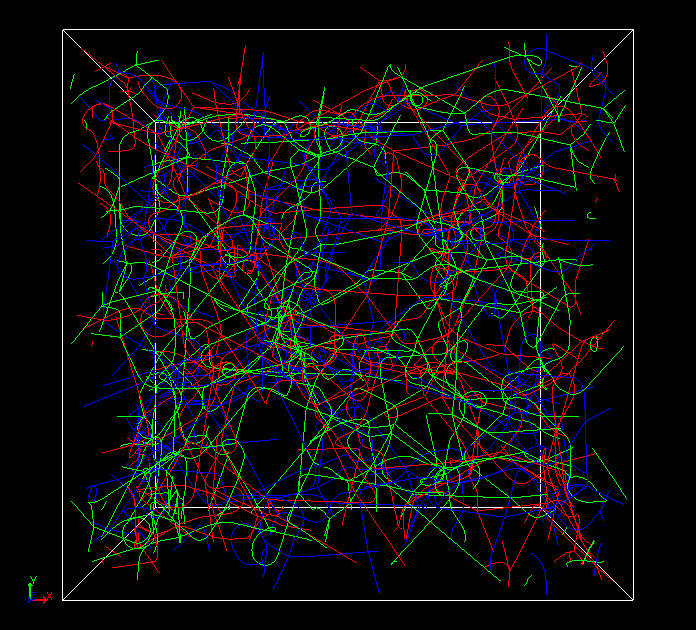
\includegraphics[width=.65\textwidth]{N48_f4_PPA.png}
				\end{center}
				
			\end{block}
			\column{.48\linewidth}
			\begin{block}{仮想的なモデル状態}
				\begin{itemize}
					\item 全ての非結合ポテンシャルを無効
					\item す抜けに設定したPPA
				\end{itemize}
				\begin{center}
					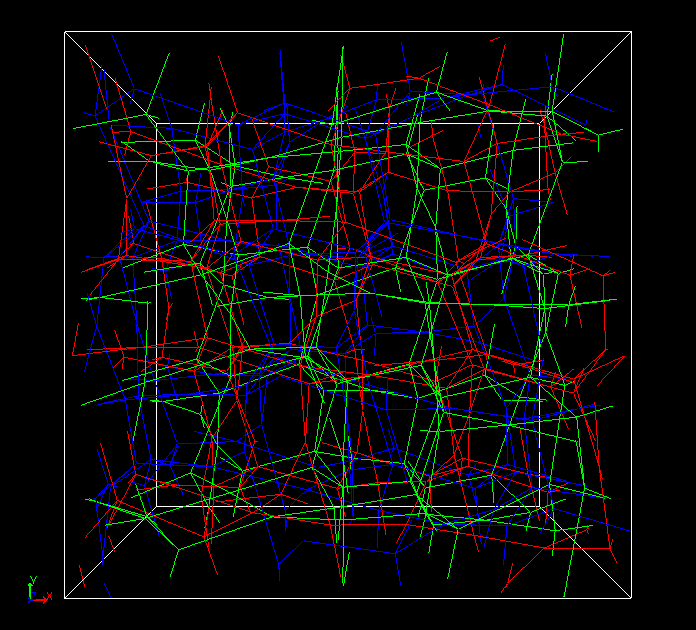
\includegraphics[width=.65\textwidth]{PPA_sunuke_NW.png}
				\end{center}
			\end{block}
		\end{columns}
        \vspace{-2mm}
        \small
		\begin{screen}
			PPA: Primitive Path Analysis\footnote{
                S. K. Sukumaran, et al., J. of Polym. Sci., Part B, 43, 917 (2005)
            }
		\end{screen}
\end{frame}



\begin{frame}
	\frametitle{ネットワーク構造でのG1-cord}
		\begin{center}
			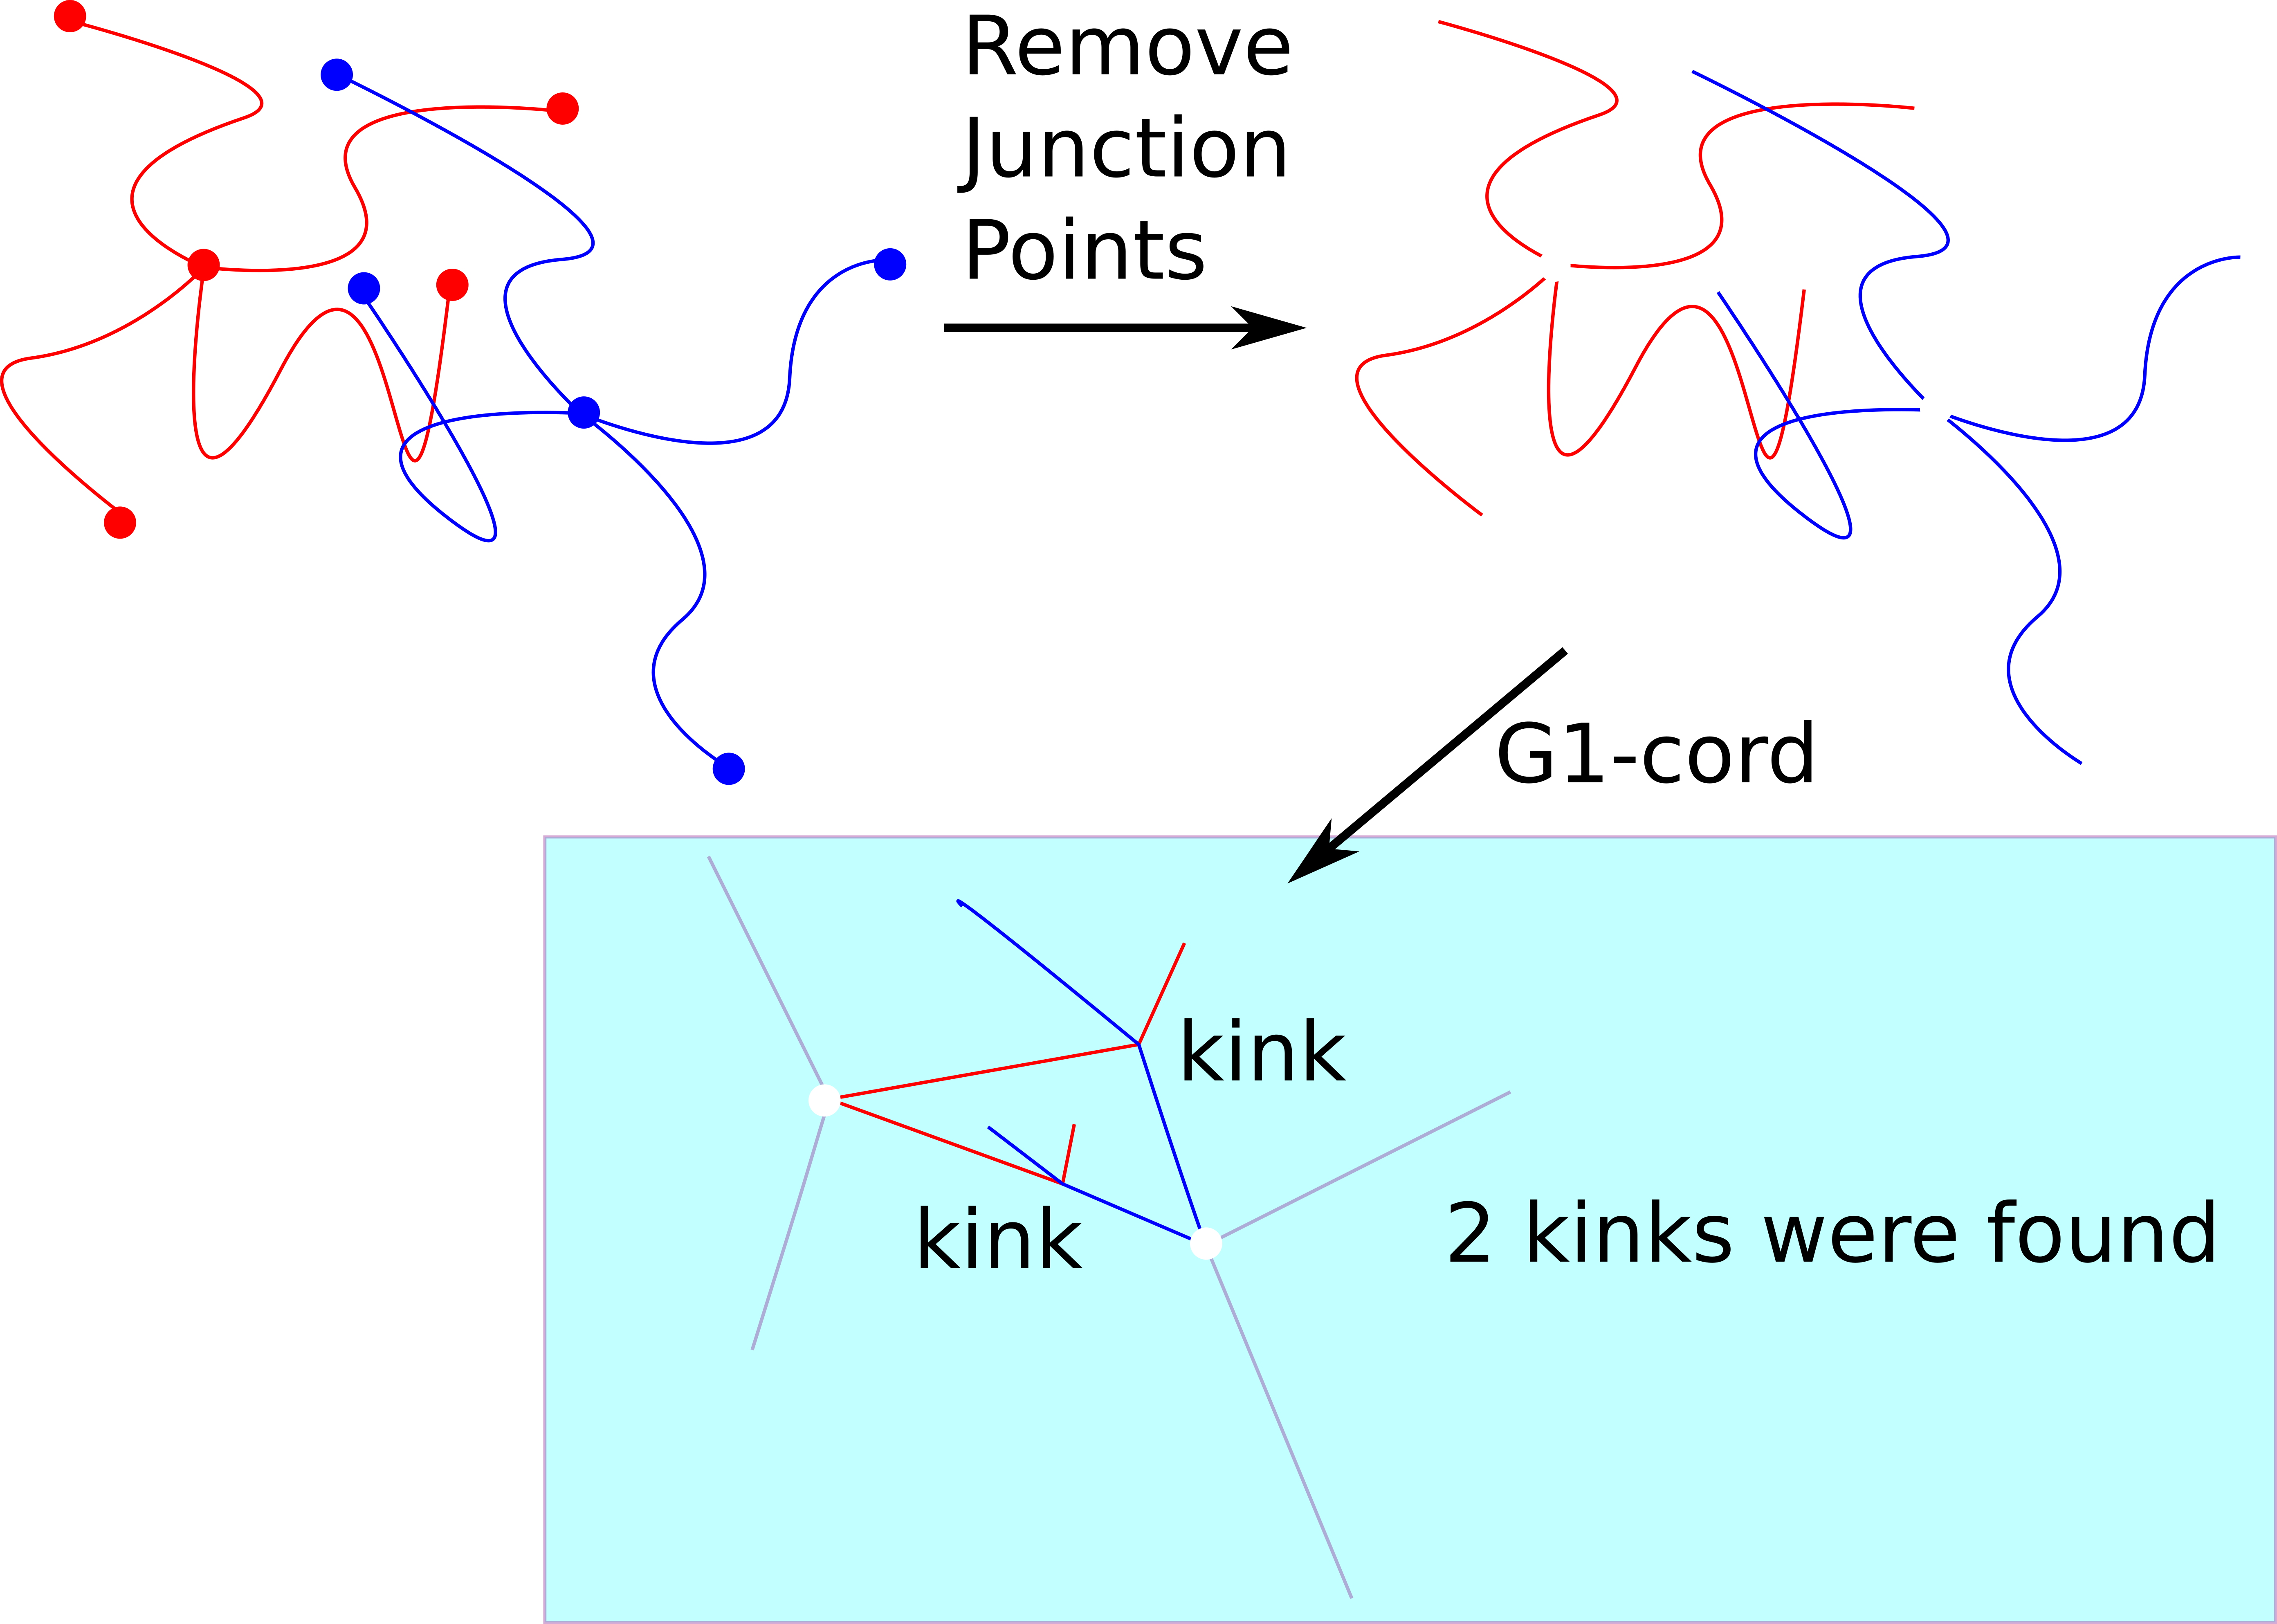
\includegraphics[width=.8\textwidth]{g1cord.png}
		\end{center}
\end{frame}


\subsection{ゴムの破断について}

% %%%%%%%%%%%%%%%%%
\begin{frame}
	\frametitle{SBRでの伸びきり効果}
		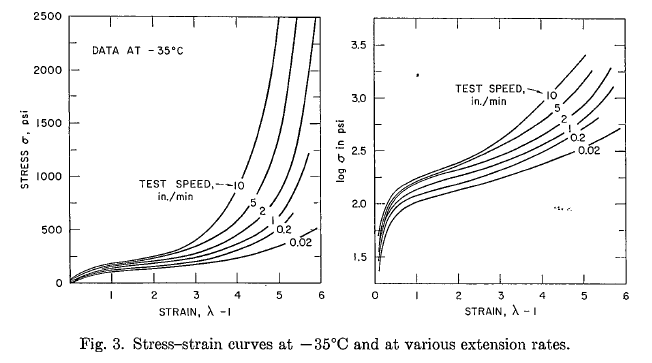
\includegraphics[width=.8\textwidth]{SBR_lowTemp_2.png}

		{\footnotesize Smith TL., Dickie RA., J. Pol. Sci. part A-2 (1969) 7 635}
		\begin{alertblock}{室温で伸び切りが出ないはずのSBR}
			\begin{itemize}
				\item 低温、高速変形でSBRでも伸びきり効果が発現
				\item 時間温度換算則で考えてみれば?
			\end{itemize}
		\end{alertblock}
\end{frame}

\begin{frame}
	\frametitle{ヒステリシスと破断エネルギーとの関係}
    \begin{alertblock}{ヒステリシス ($H$) と破断エネルギー ($U_B$) との関係}
        \vspace{-5mm}
        \begin{align*}
            &U_B = 3.9 H^{2/3}\\
            &\text{for SBR over a temperature range of -40 to 144$^o$C}
        \end{align*}
        
    \end{alertblock}

    % \vspace{2mm}
    \begin{center}
        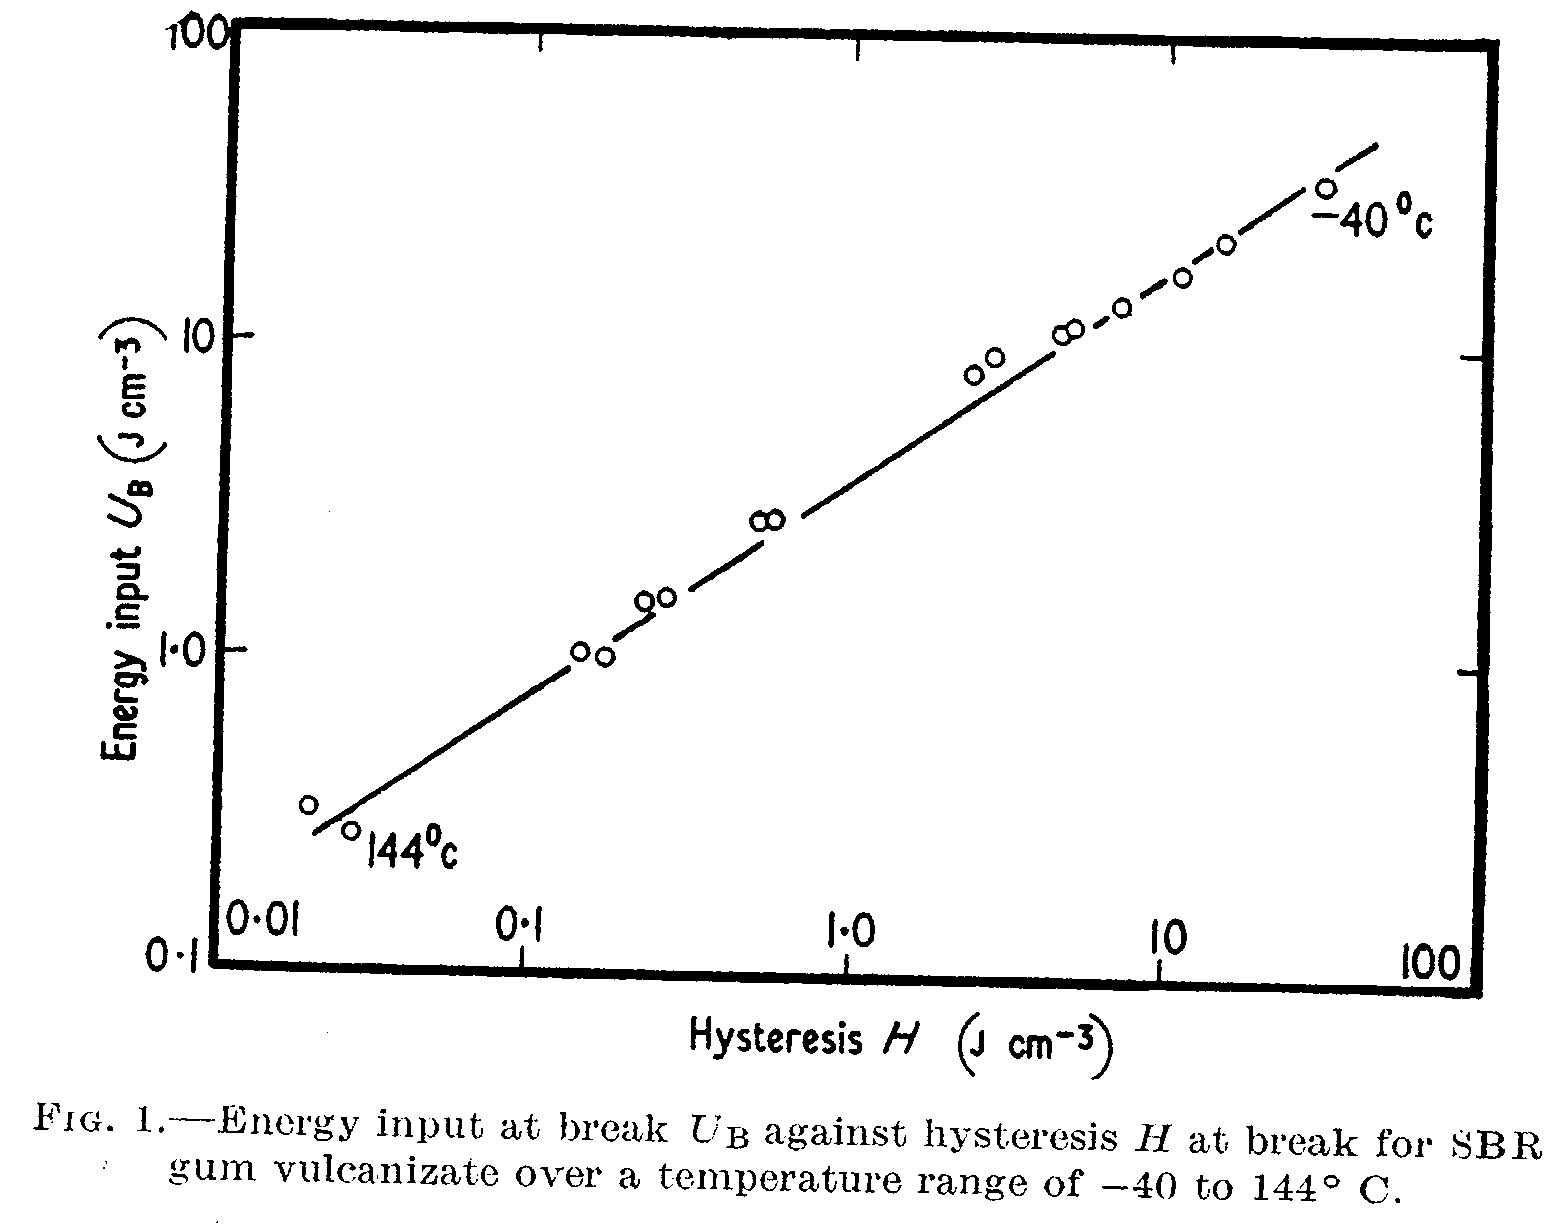
\includegraphics[width=.52\textwidth]{hyst_break.png}
    \end{center}
	
    \vspace{-3mm}
	{\footnotesize K. A. Grosch et al. Rub. Chem. and Tech.41, 1157 (1968)}
\end{frame}

\subsection{補足のデータ}

\begin{frame}
	\frametitle{四分岐ネットワークの平衡構造 (NVT)}
		\begin{columns}[T, onlytextwidth]
			\column{.48\linewidth}
				\begin{block}{四分岐ネットワークの作成}
					\begin{itemize}
						\item ストランドの末端間距離がホモポリマーと同等となるように、
						\item セグメント数 N=48 のストランドを選択し、
						\item 多重度を 3 とした四分岐ネットワークを作成。
						% \item 十分に初期緩和
					\end{itemize}
					\begin{center}
						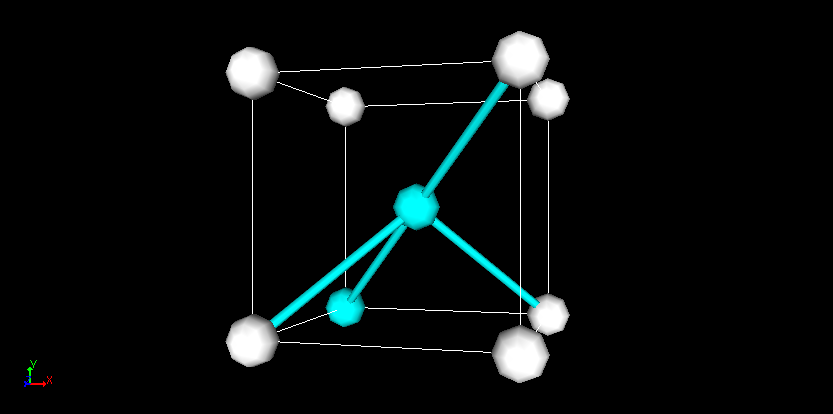
\includegraphics[width=.6\textwidth]{8_4.png}
					\end{center}
				\end{block}
			\column{.5\linewidth}
				\footnotesize
				\begin{itemize}
					\item 鎖に沿ったセグメント間\\距離のトラジェクトリ
					
					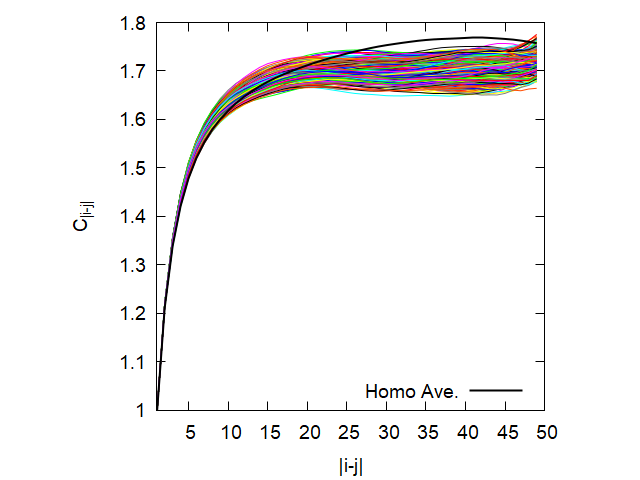
\includegraphics[width=.64\textwidth]{N48_f4_CN.png}

					\item 末端間距離の分布関数
					
					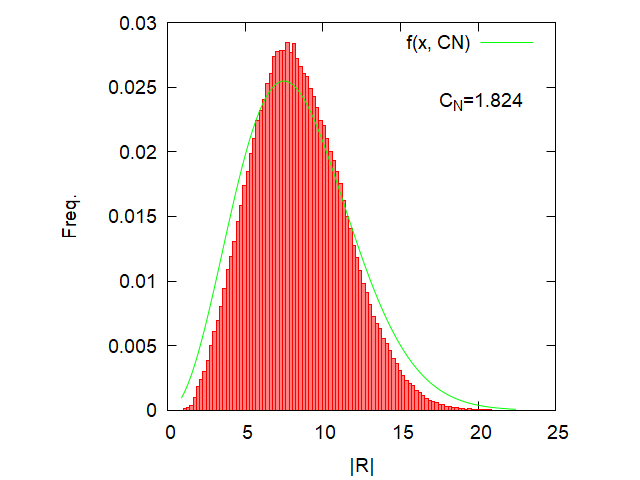
\includegraphics[width=.64\textwidth]{R_N48_f4.png}
				\end{itemize}
		\end{columns}
\end{frame}

\begin{frame}
	\frametitle{四分岐ネットワークの力学応答}
		\begin{columns}[T, onlytextwidth]
			\column{.48\linewidth}
				\begin{block}{一軸伸張結果}
					\begin{itemize}
						\item 伸張速度の低下によりネオフッキアンに漸近
						\item ANMよりも応力は高い
					\end{itemize}
					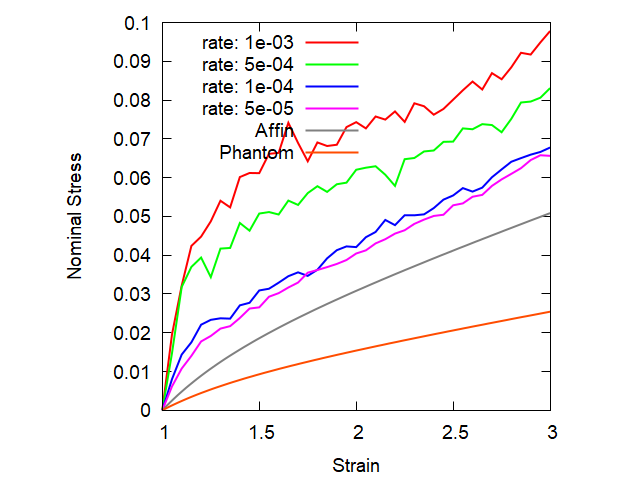
\includegraphics[width=\textwidth]{N48_C4_M3.png}
				\end{block}
				
			\column{.48\linewidth}
				\begin{block}{Moony-Rivlin Plot}
					\begin{itemize}
						\item Shear Rate = 1e-4
						
						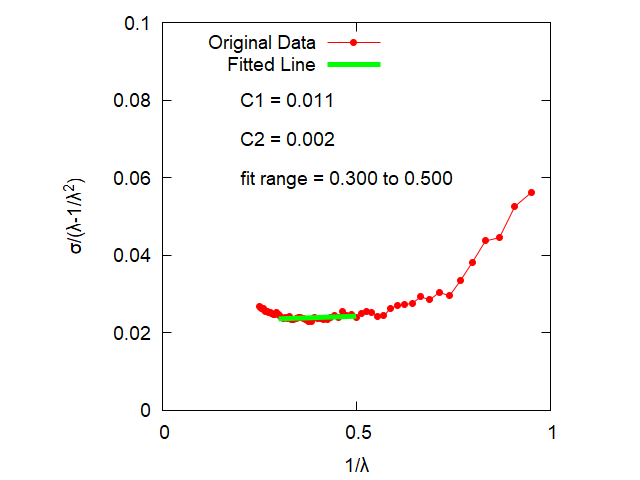
\includegraphics[width= .6\textwidth]{MR_rate_1e-04.png}
						\item Shear Rate = 5e-5
						
						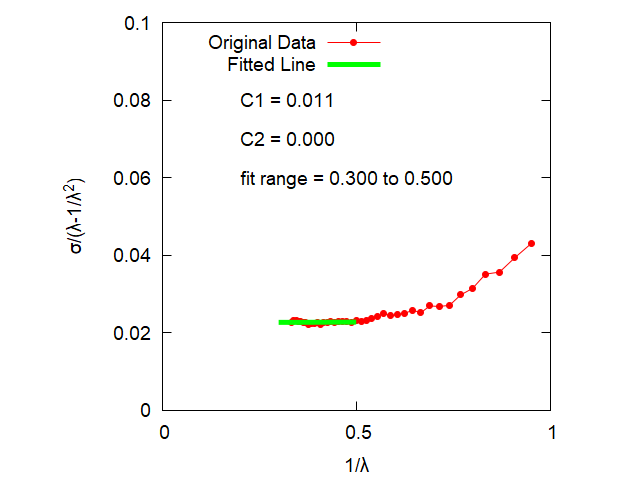
\includegraphics[width= .6\textwidth]{MR_rate_5e-05.png}
					\end{itemize}
					
				\end{block}
		\end{columns}
\end{frame}

\begin{frame}
	\frametitle{四分岐ネットワークの力学応答}
		\begin{columns}[T, onlytextwidth]
			\column{.48\linewidth}
				\begin{block}{一軸伸張結果}
					\begin{itemize}
						\item 伸張速度の低下によりネオフッキアンに漸近
						\item ANMよりも応力は高い
					\end{itemize}
					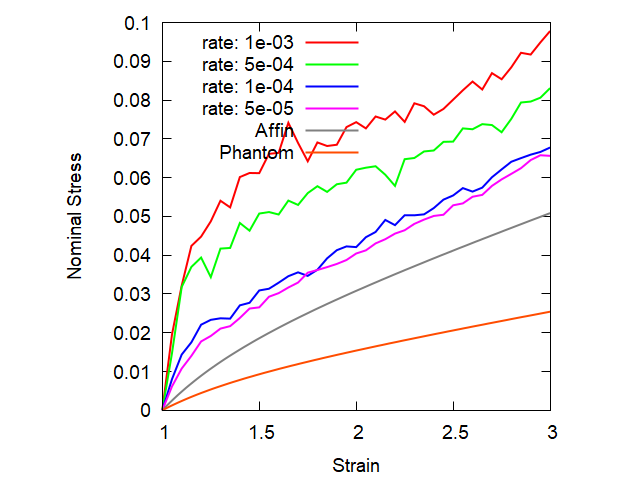
\includegraphics[width=\textwidth]{N48_C4_M3.png}
				\end{block}
				
			\column{.48\linewidth}
				\begin{block}{応力緩和関数 $G(t)$}
					\begin{itemize}
						\item ステップ変形($\lambda=2.0$)
						\item 最長緩和の長時間化
						\item ANM よりも高弾性率
					\end{itemize}
					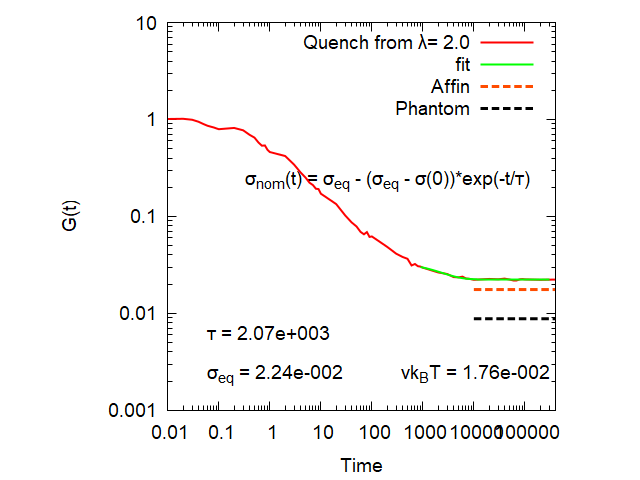
\includegraphics[width=\textwidth]{gt_N48_C4_M3.png}
				\end{block}
		\end{columns}
\end{frame}
\end{document}
